\documentclass{report}
% Include all project wide packages here.
\usepackage{fullpage}
\usepackage[style=ieee]{biblatex}
\usepackage[dutch]{babel}

\renewcommand{\familydefault}{\sfdefault}

\setmainfont[Ligatures=TeX]{Myriad Pro}
\setmathfont{Asana Math}
\setmonofont{Lucida Console}

\usepackage{titlesec, blindtext, color}
\definecolor{gray75}{gray}{0.75}
\newcommand{\hsp}{\hspace{20pt}}
\titleformat{\chapter}[hang]{\Huge\bfseries}{\thechapter\hsp\textcolor{gray75}{|}\hsp}{0pt}{\Huge\bfseries}
\renewcommand{\familydefault}{\sfdefault}
\renewcommand{\arraystretch}{1.2}
\setlength\parindent{0pt}

%For code listings
\definecolor{black}{rgb}{0,0,0}
\definecolor{browntags}{rgb}{0.65,0.1,0.1}
\definecolor{bluestrings}{rgb}{0,0,1}
\definecolor{graycomments}{rgb}{0.4,0.4,0.4}
\definecolor{redkeywords}{rgb}{1,0,0}
\definecolor{bluekeywords}{rgb}{0.13,0.13,0.8}
\definecolor{greencomments}{rgb}{0,0.5,0}
\definecolor{redstrings}{rgb}{0.9,0,0}
\definecolor{purpleidentifiers}{rgb}{0.01,0,0.01}


\lstdefinestyle{csharp}{
language=[Sharp]C,
showspaces=false,
showtabs=false,
breaklines=true,
showstringspaces=false,
breakatwhitespace=true,
escapeinside={(*@}{@*)},
columns=fullflexible,
commentstyle=\color{greencomments},
keywordstyle=\color{bluekeywords}\bfseries,
stringstyle=\color{redstrings},
identifierstyle=\color{purpleidentifiers},
basicstyle=\ttfamily\small}

\lstdefinestyle{c}{
language=C,
showspaces=false,
showtabs=false,
breaklines=true,
showstringspaces=false,
breakatwhitespace=true,
escapeinside={(*@}{@*)},
columns=fullflexible,
commentstyle=\color{greencomments},
keywordstyle=\color{bluekeywords}\bfseries,
stringstyle=\color{bluestrings},
identifierstyle=\color{purpleidentifiers}
}

\lstdefinestyle{vhdl}{
language=VHDL,
showspaces=false,
showtabs=false,
breaklines=true,
showstringspaces=false,
breakatwhitespace=true,
escapeinside={(*@}{@*)},
columns=fullflexible,
commentstyle=\color{greencomments},
keywordstyle=\color{bluekeywords}\bfseries,
stringstyle=\color{redstrings},
identifierstyle=\color{purpleidentifiers}
}

\lstdefinestyle{xaml}{
language=XML,
showspaces=false,
showtabs=false,
breaklines=true,
showstringspaces=false,
breakatwhitespace=true,
escapeinside={(*@}{@*)},
columns=fullflexible,
commentstyle=\color{greencomments},
keywordstyle=\color{redkeywords},
stringstyle=\color{bluestrings},
tagstyle=\color{browntags},
morestring=[b]",
  morecomment=[s]{<?}{?>},
  morekeywords={xmlns,version,typex:AsyncRecords,x:Arguments,x:Boolean,x:Byte,x:Char,x:Class,x:ClassAttributes,x:ClassModifier,x:Code,x:ConnectionId,x:Decimal,x:Double,x:FactoryMethod,x:FieldModifier,x:Int16,x:Int32,x:Int64,x:Key,x:Members,x:Name,x:Object,x:Property,x:Shared,x:Single,x:String,x:Subclass,x:SynchronousMode,x:TimeSpan,x:TypeArguments,x:Uid,x:Uri,x:XData,Grid.Column,Grid.ColumnSpan,Click,ClipToBounds,Content,DropDownOpened,FontSize,Foreground,Header,Height,HorizontalAlignment,HorizontalContentAlignment,IsCancel,IsDefault,IsEnabled,IsSelected,Margin,MinHeight,MinWidth,Padding,SnapsToDevicePixels,Target,TextWrapping,Title,VerticalAlignment,VerticalContentAlignment,Width,WindowStartupLocation,Binding,Mode,OneWay,xmlns:x}
}

%defaults
\lstset{
basicstyle=\ttfamily\small,
extendedchars=false,
numbers=left,
numberstyle=\ttfamily\tiny,
stepnumber=1,
tabsize=4,
numbersep=5pt
}
\addbibresource{../../library/bibliography.bib}

\title{EPO-2: Mid-term Design Report - routevolger}
\author{Tijmen Witte}

\begin{document}

\chapter{Routevolger}
\label{ch:routevolger}

Als er naar het grid wordt gekeken in hoofdstuk \ref{ch:probleemstelling} kan men zien dat er meer bij komt kijken dan alleen het volgen van een lijn, zoals in het vorige hoofdstuk beschreven is.
Doordat er kruispunten aanwezig zijn, ontstaan er drie mogelijke wegen die de robot kan nemen.
Bij het volgen van de route moet de robot rekening houden met de kortste route en hier op inspelen.
Mochten er mijnen op de route liggen dan moet de robot op het moment dat hij deze herkent terugrijden, zodat de lichtsensoren weer voor het kruispunt zitten.
Is dit niet het geval dan slaat hij het kruispunt over, waardoor hij letterlijk de weg kwijt is.

\section{Eisen}
\begin{itemize}
	\item De robot moet in staat zijn een door de PC berekende route te rijden
	\item Dit moet zo tijdsefficiënt mogelijk gebeuren
	\item Tijdens dit proces moet gereageerd kunnen worden op mijnen
\end{itemize}

\section{Ontwerp}
Het proces wat zich afspeelt wanneer de robot een route volgt is vanzelfsprekend af te leiden uit de VHDL-code, maar kan als volgt kort samengevat worden:

\begin{itemize}
	\item De robot komt op een kruispunt en vraagt de PC wat hij moet doen
	\item De PC antwoord met een instructie, bestaande uit een richting: vooruit, links, rechts of omdraaien
		\begin{itemize}
			\item Wanneer de robot op het punt staat een controlepost in te rijden en daarna door moet naar andere posten volgt direct op de richting ook een continue-signaal
			\item Wanneer de robot op het punt staat de laatste controlepost in te rijden, volgt direct op deze instructie een done-signaal
		\end{itemize}
	\item De robot antwoord dat hij de instructie ontvangen heeft
	\item De robot komt dan bij de zwarte cirkel die aangeeft waar al dan niet een mijn ligt en detecteert deze
		\begin{itemize}
			\item Als hier een mijn ligt stuurt hij dat naar de PC
			\item Als hier geen mijn ligt stuurt de robot de PC dat hij halverwege is en rijdt hij door
		\end{itemize}
	\item Als de robot een mijn detecteerde rijdt hij achteruit terug naar het vorige kruispunt en vraagt opnieuw om instructie en de cyclus wordt opnieuw ingezet
	\item Als de robot geen mijn detecteerde en doorreed komt hij bij het volgende kruispunt, waar hij om instructie vraagt en de cyclus opnieuw begint
\end{itemize}

Deze instructies zijn conform het gebruikte protocol, zoals te vinden in bijlage \ref{app:communicatie} tabel \ref{tab:comProtocol}.

Het ontwerpen van de routevolger in zijn huidige staat was een moeizaam proces. Zo zijn we bijvoorbeeld tegen het probleem aan gelopen dat de robot zo scherp draaide dat hij de lijn waar hij naar toe moest miste en dus in feite 180 graden draaide. Na aanpassingen kwam het voor dat bochten goed gemaakt werden, alleen met een dusdanige zwaai dat eventuele mijnen gemist werden. De uiteindelijke oplossing was om de robot eerst een stuk vooruit te laten rijden door middel van een vertraging en hem daarna om zijn as te laten draaien door de motoren met maximale snelheid in tegengestelde richting te laten draaien. Het resultaat mocht er zijn.

In eerste instantie hebben we ook gekozen om 180 graden te draaien op het moment dat de robot een mijn tegenkomt. Omdat dit vrij foutgevoelig bleek te zijn, is later overgestapt op een ontwerp waarin de robot niet omdraait, maar achteruit terugrijdt naar het vorige kruispunt. Omdat de robot hiervoor niet hoeft te roteren en de lineaire verplaatsing ook slechts enkele centimeters bedraagt is de kans dat er iets fout gaat waardoor de robot bijvoorbeeld de lijn niet meer volgt een stuk kleiner geworden.

\section{Implementatie}
Onze implementatie van de routevolger en de bijbehorende lijnvolger zijn te vinden in bijlage \ref{appsec:controller.vhdl}, als onderdeel van de overkoepelende controller, waar uitgebreid op ingegaan wordt in hoofdstuk \ref{ch:controller}.

\section{Test}
We hebben een eigen testveld gemaakt (figuur \ref{fig:testfield}), om de robot te testen. Dit had als voordeel datt we niet steeds naar het grote testveld hoefden te gaan met laptop en robot om kleine aanpassingen te testen.
Door de robot van punt $1_B$ naar punt $2_A$ te laten rijden, hebben we kunnen testen of de robot de kruispunten herkende en of hij de bochten in de juiste richting nam. Tevens simuleerde deze route een route van controlepost naar controlepost op het echte veld.
Nadat de mijnendetector was aangesloten, hebben we mijnen geplaatst op de middenstukken en konden we testen of de robot op het juiste moment terugreed als hij een mijn had gedetecteerd. Na het terugrijden zouden de lichtsensoren weer voor het kruispunt recht op de lijn moeten zitten.
Bij elke schijnbare vooruitgang hebben we natuurlijk ook getest op het grote veld met verschillende situaties en routes.

\begin{figure}[H]
	\centering
	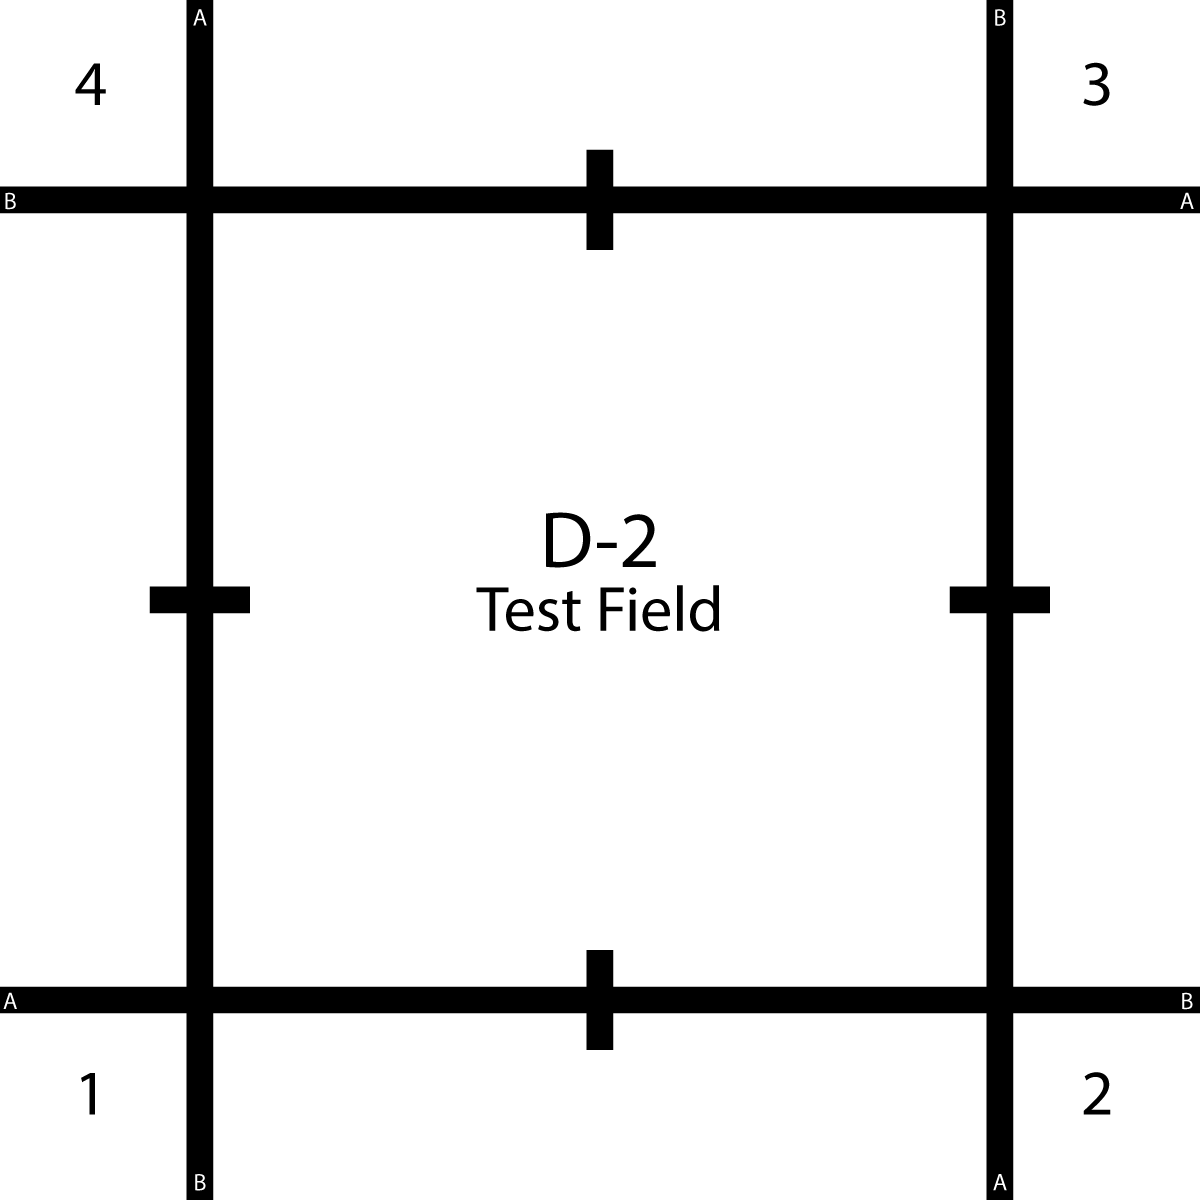
\includegraphics[width=0.5\textwidth]{d-2_test_field.png}
	\caption{Zelf gemaakt testveld voor EPO-2}
	\label{fig:testfield}
\end{figure}

\section{Discussie}

Zoals eerder vermeld is het ontwerpproces niet gemakkelijk geweest, we zijn echter toch tot een werkend resultaat gekomen. Omdat deze implementatie pas de dag van de inleverdatum van dit verslag is gemaakt, hebben we helaas niet veel kunnen doen aan stabiliteitstesten. Perfect zal het dus niet zijn, maar het is wel de meest stabiele implementatie die wij in de afgelopen weken hebben gemaakt. Desalniettemin is aan alle eisen voldaan.

Om even kort te reflecteren op het proces, zouden we kunnen stellen dat het ons veel tijd had bespaard als er wat zorgvuldiger was gedaan tijdens het programmeren en testen. Als voorbeeld hebben we de nodige tijd verloren, toen de robot het niet leek te doen. Dit bleek echter niet te komen door een bug of glitch, maar omdat er een schakelaar verkeerd stond ingesteld.
Fouten maken is natuurlijk menselijk, maar het aantal fouten had kleiner kunnen zijn.

\end{document}
